\documentclass{whutmod}
\usepackage{metalogo}
\usepackage{float}
\usepackage{subfigure} 
\usepackage{url}
\usepackage{booktabs}
\bibliographystyle{unsrt}
\team{23}
\membera{刘子川}
\joba{编程}
\memberb{程宇}
\jobb{建模}
\memberc{陈荣兴}
\jobc{建模}
\hypersetup{
	colorlinks=true,
	linkcolor=black
}

\title{基于因子分析与灰色关联分析对武汉市人才吸引力的量化评价}
\tihao{4} 

\begin{document}

	%\maketitle
	\begin{abstract}

本文构建\textbf{灰色马尔科夫模型},预测2019年全国感染该疾病的发病人数和死亡人数。再通过该预测模型,预测各个人群与地区的发病率特征。将发病率特征带入\textbf{TOPSIS模型},得到防控排名前$3$位的重点区域和重点人群。
~\\

针对问题一,在传统\textbf{灰色预测模型}的基础上,附加\textbf{马尔科夫链}校正预测结果误差,得到\textbf{灰色马尔科夫模型},预测2019年传染病数据。本组首先建立传统\textbf{GM(1,1)}模型,预测分析2004-2019年该流行病的发病人数和死亡人数。再通过\textbf{马尔科夫模型},由2004-2016年的数据模拟残差在各个区间的分布,计算2017-2019年预测残差的期望值。最后将预测结果与残差期望做差,校正传统灰色预测的固有偏差。求得2019年患病人数\textbf{740960}人、死亡人数\textbf{2211}人。	
~\\

针对问题二,基于问题一模型,预测各人群、各地区的患病情况特征,再通过\textbf{TOPSIS}法选出各人群、各地区排名前三的重点防控对象。首先将附件中各个省市与各个职业的发病人数、死亡人数数据,带入问题一的灰色马尔科夫模型中。预测出2019年发病人数、死亡人数,发病人数增长率、死亡人数增长率和死亡率。并将上述五个指标带入TOPSIS综合评价模型,分别赋予权重\textbf{0.15、0.3、0.15、0.3和0.1},,计算各人群、各地区的综合评价得分,选取排序前三位的省市——\textbf{新疆}、\textbf{西藏}和\textbf{青海}和排序前三位的职业——\textbf{农民}、\textbf{家政家务}和\textbf{退休人员}分别作为重点防控区域和重点防控人群。
~\\

针对问题三,本组爬取网络各省市经济发展数据,并通过灰色关联度分析筛选合适指标,最后通过\textbf{支持向量回归(SVR)}建立该传染病与经济发展的数学模型。  首先收集$31$个省市各年度的经济发展数据。通过灰色关联度分析,得到经济指标中与患病人数和死亡人数灰色关联度排名前三的是\textbf{人均GDP}、\textbf{居民消费水平}和\textbf{一般预算收入}。再基于\textbf{SVR回归}得出经济指标分别对于患病人数和死亡人数的回归分析模型。
~\\

针对问题四,基于问题二中的传染病传播模型和\textbf{TOPSIS评价模型}以及对各地区和不同人群的综合评价排名,并结合问题三中利用\textbf{SVR回归}判断传染病与经济发展关系模型的结果与分析,给卫生健康委员会相关部门写一封公开信。

本文中所提到的模型优点主要有两点:一、利用马尔可夫模型改进后的灰度预测值与实际值拟合度更高,波动性保持一致;二、针对支持向量回归参数选取,利用灰色关联度筛选合适指标,相较于主观选取指标具有客观性、严谨性。

	
  
\keywords{马尔可夫模型\quad  灰度预测\quad  TOPSIS综合评价\quad 支持向量回归\quad }


	\end{abstract}
	%目录
	\tableofcontents
	\newpage	%换页符
	
	\section{问题重述}	
	\subsection{问题背景}
    随着全球化的进程,人类活动范围日益扩大,人群流动频繁,传染病可在大范围内迅速传播,是对人类社会存在威胁的公共卫生问题。在疾病控制实际工作中,疾病的发病与流行趋势分析是极其重要的一环,科学、准确的分析能对卫生行政部分制定疾病预防与控制策略产生重要的影响,传染病早期预警将大大降低传染病的社会经济危害。
    
    为了提高某传染病疫情和突发公共卫生事件报告的质量和时效,加强对全国感染病人的诊断、治疗和督导管理,卫生部建立了全国监管机制,及时通报相关病情和相关数据,并通过对疫情数据的动态分析,建立该传染病防治工作督导检查、防治效果评价和制定防治对策和策略,控制并逐渐消灭该传染病。构建预测模型从早期探测到传染病的爆发并及时预警,采取应对措施,是目前传染病防控的重要手段,具有重要的实际意义。
    
    

	\subsection{问题概述}
    围绕相关附件和条件要求,研究海运装载行动输送兵力任务的合理安排,依次提出以下问题:
		 
	
	\textbf{问题一:}根据合适的指标建立模型,分析流行病在2004-2016年的变化趋势,并预测2019年全国感染该病的发病数和死亡数。
	
	\textbf{问题二:}基于2004-2016年每隔三年的不同地区的和职业分类的数据,建立疾病传播模型,并预测2019年传染病重点防控前3名的区域和职业人群。
		
	\textbf{问题三:}结合地区经济发展的相关数据,选择一个角度建立传染病与经济发展相关的模型,并分析结论。
	
	\textbf{问题四: }综合模型结果及分析,给卫生健康委员会相关部门写一封公开信,谈谈对传染病疫情防治的看法和建议。
	
	
	\section{模型假设}
	\begin{itemize}                                             
		\item [(1)] 为保证预测结果精确性,假设题目所给出数据真实可信。
		\item [(2)] 假设重点防控的区域和人群中的发病人数和死亡人数的增长率比其基数更加重要。
		\item [(3)] 假设与经济发展无关的该传染病的其它影响因素可以忽略不计。
		\item [(4)]	忽略地区之间的人口流动对患病数和死亡数变化的影响。
	\end{itemize}
	

	\section{符号说明}
	\begin{table}[H]
	\label{biao} \centering
	\begin{tabular}{cc}
		\toprule[1.5pt]
		\multicolumn{1}{m{5cm}}{\centering 符号} & \multicolumn{1}{m{5cm}}{\centering 说明} \\
		\midrule[1pt]		
		$X^{(i)}$  & 人数时间序列  \\ 
		$a$  &  发展灰度 \\ 
		$u$  &  内生控制灰度\\
		$\widehat{\alpha}$  &  待估参数向量 \\ 
		$\varepsilon$ & 残差序列\\
		$P$	 &  状态转移矩阵  \\ 
		$E_{k}$ &  状态区间 \\ 
	%	$n_{Ek}$	 &  状态$E_{k}$出现的次数 \\ 
		$\eta $  &   误差期望\\ 
		$\overline{x}(k)$  &  灰色马尔可夫组合预测值\\	
		$\widehat{x}(k)$ & 灰色预测值\\
		$t_{0}'$ &  初始状态概率向量\\ 
		$A$ & 职业多属性决策矩阵\\
		$B$ & 规范化决策矩阵\\
		$W$ & 权重向量\\
		$C$  & 加权规范矩阵\\
		$C^{*}$ & 正理想解\\
		$C^{0}$ & 负理想解\\
		$d_{i}$ & 属性决策向量\\
		$ f_{i}^{*}$ &  综合评价指数\\
		$ \delta_{i}$ &发病人数增长率 \\
		$ \eta_{i}$    &患病人口死亡率 \\
		\bottomrule[1.5pt]
	\end{tabular}
\end{table}

	\section{问题一模型的建立与求解}
    \subsection{问题描述与分析}

    问题一要求,根据附件中2004年至2016年的流行病相关数据,预测2019年全国感染该疾病的发病人数和死亡人数。本组首先选择合适的指标后建立\textbf{灰色预测}模型,预测分析2004-2019年该流行病的发病人数和死亡人数。再通过\textbf{马尔科夫模型},由2004-2016年的数据模拟残差在各个区间的分布,计算2017-2019年预测残差的期望值。最后将预测结果与残差期望做差,\textbf{校正}传统灰色预测的固有偏差,经过两种模型的有效结合达到科学预流行病的未来发展趋势。其问题一思维流程图如图~\ref{lct}~所示:

       \begin{figure}[H]
   	\centering
   	
\includegraphics[width=\textwidth]{figures/lctc.png}
   	\caption{问题一思维流程图}\label{lct}
   \end{figure}

   
	    \subsection{模型的建立}
	    \subsubsection{灰度预测GM(1,1)}
	    设2004-2016年总发病人数为时间序列:
	     \begin{gather*}
	    X^{(0)}=[x^{(0)}(1),x^{(0)}(2),\cdots,x^{(0)}(13)]
	    \end{gather*}
	    
	    通过一次累加生成1-AGO序列:
	    \begin{gather*}
	    X^{(1)}=[x^{(1)}(1),x^{(1)}(2),\cdots,x^{(1)}(13)]
	    \end{gather*}
	    式中:$x^{(1)}(k)=\sum_{i=1}^{k}x^{(1)}(i),k=1,2,\cdots,13$。
	    
	    根据1-AGO序列建立微分方程为\cite{bib:one}:
	     \begin{gather}\label{333}
	    \frac{d X^{(1)}}{dt}+a X^{(1)} = u
	     \end{gather}
	     式中:$a$称为发展灰度,$u$称为内生控制灰度。设$\widehat{\alpha}$为待估参数向量,且$\widehat{\alpha }=[a,u]^T$,利用最小二乘法求出:
	     \begin{gather}
	     \widehat{\alpha }=(B^TB)^{-1}B^{T}Y_{n}
	     \end{gather}

	     
	     求解方程(~\ref{333}~),可得第$k+1$年传染病发病数\textbf{初步预测模型}为:

	     \begin{gather}
	     \widehat{X}(k+1)=[X^{(0)}(1)-\frac{u}{a}]e^{-ak}+\frac{u}{a},k=1,2,\cdots,16
	     \end{gather}
	     
	     同理将死亡数作为向量$X^{(0)}=[x^{(0)}(1),x^{(0)}(2),\cdots,x^{(0)}(13)]$带入模型可求得2017-2019年死亡数灰度预测值。
	     \subsubsection{马尔科夫模型校正}
	     利用马尔科夫模型对GM(1,1)预测误差项的状态及状态概率进行预估,并利用预测状态的期望值对GM(1,1)预测值进行修正\cite{bib:2}。用2004-2016年预测数据与真实数据残差进行状态划分,设残差序列为:
	     \begin{gather*}
	    \varepsilon =[\varepsilon(1) ,\varepsilon(2), \cdots,\varepsilon(13)]
	     \end{gather*}
	     
	    最大残差绝对值为$\delta _{max}=\underset{1\leqslant i\leqslant13 }{max}\left | \varepsilon(i) \right |$,将预测误差化均分为三个状态。令$\lambda =\frac{\delta _{max}}{6}$。状态分别为$E_{1}:(-3\lambda,-\lambda)$、$E_{2}:(-\lambda,\lambda)$和$E_{1}:(\lambda,3\lambda)$。其中初始状态概率向量计算公式为:
	    
	   \begin{gather}
	 \left\{\begin{matrix}
	 t_{0}=[p_{E1},p_{E2},p_{E3}]\\ 
	 p_{Ek}=\frac{n_{Ek}}{13}
	 \end{matrix}\right.
	  \end{gather}
	  式中:$n_{Ek}$是状态$E_{k}$在2004-2016年内出现的次数,以状态$E_{k}$出现的频率代替其出现的概率$p_{Ek}$。且构建状态转移矩阵为:
	   \begin{gather*}
	  P=\left(\begin{array}{lll}{P_{11}} & {P_{12}} & {P_{13}} \\ {P_{21}} & {P_{22}} & {P_{23}} \\ {P_{31}} & {P_{32}} & {P_{33}}\end{array}\right)
	  \end{gather*}
	   式中:$P_{ij}$是由状态$E_{i}$经过一个时期转移到$E_{j}$的转移概率。
	   
	   即马尔科夫模型可表示为:	  
	   \begin{gather}
	   t_{k+1}=t_{k} \cdot p
	  \end{gather}
	  
	  设状态区间的中间值分别为$\overline{E}_{1}$、$\overline{E}_{2}$和$\overline{E}_{3}$,即第k年GM(1,1)的误差期望为:
	   \begin{gather}
\eta =\begin{bmatrix}
p_{E1} & p_{E2} & p_{E3}
\end{bmatrix} \cdot\begin{bmatrix}
\overline{E}_{1}\\ 
\overline{E}_{2}\\ 
\overline{E}_{3}
\end{bmatrix}
	  \end{gather}
	  
	  当第$k$年的患病人数的GM(1,1)预测值为$\widehat{x}(k)$时,\textbf{修正后的灰色马尔可夫组合预测}模型$\overline{x}(k)$可以记作:
	     \begin{gather}
	     \overline{x}(k) =\widehat{x}(k)-\eta
	   \end{gather}
	   \subsubsection{预测结果评价指标}
	   均方根误差(RMSE)、平均相位误差绝对值(MAPE)和纳什效率系数(NSE)三者是常用来衡量预测结果的指标。RMSE能评价患病人数和死亡人数中高值的预测结果,其计算公式为:

	    \begin{gather*}
	   \operatorname{RMSE}=\sqrt{\frac{1}{n} \sum_{i=1}^{n}\left(y_{i}-y_{i}^{*}\right)^{2}}
	   \end{gather*}
	   

	   均方根误差越小,表明模型可靠性越高,结果越准确。
	    
	     MAPE用来评价预测数据中平稳部分的预测结果,其计算公式为:
	    \begin{gather*}
\mathrm{MAPE}=\frac{1}{n} \sum_{i=1}^{n}\left|\frac{y_{i}-y_{i}^{*}}{y_{i}}\right| \times 100 \%
	     \end{gather*}
	     MAPE所求值为绝对值,是一个相对指标,当两个MAPE值进行比较时,值越小的说明模型可靠性越高。
	     
	       NSE可以用来评价模型的预测能力,其计算公式如下:
	       	\begin{gather*}
\mathrm{NSE}=1-\frac{\sum_{i=1}^{n}\left(y_{i}-y_{i}^{*}\right)^{2}}{\sum_{i=1}^{n}\left(y_{i}-\overline{y}\right)^{2}}       
	       \end{gather*}
	       求得NSE值越接近$1$,表示模型质量越好,模型可信度越高。接近$0$,表示模拟结果接近观测值的平均水平,即总体结果可信,但模拟误差较大。远远小于$0$,则模型是不可信的。
	      
	 
	         
	\subsection{灰色马尔可夫模型的求解}   
	  通过GM(1,1)计算2004-2016年发病人数预测值得到灰度预测解如下:


	  	  \begin{gather}
	  \widehat{X}(k+1)=-2527359e^{-0.037k}+3497638,k=1,2,\cdots,16
	  \end{gather}

	  其误差状态区间如表~\ref{ff}~所示:
	  	 \begin{table}[H]
	  	\centering\caption{发病人数状态区间划分}\label{ff}
	  	\begin{tabular}{cccc}
	  		\toprule[1.5pt]
	  		\multicolumn{1}{m{2cm}}{\centering 状态}
	  		& \multicolumn{1}{m{3cm}}{\centering $E_{1}$}
	  		& \multicolumn{1}{m{3cm}}{\centering $E_{2}$}
	  		& \multicolumn{1}{m{3cm}}{\centering $E_{3}$}
	  		\\
	  		\midrule[0.5pt]
	  		残差区间 &  $[-66389,-22130]$  &$(-22130,22130]$ & $(22130,66389]$   \\ 
	  		\bottomrule[1.5pt]	
	  	\end{tabular}
	  \end{table}  
	  根据误差区间范围,将2004-2016年发病人数预测值归类于误差区间如表~\ref{fff}~所示:
	  \begin{table}[H]
	  	\centering\caption{发病人数误差状态区间}\label{fff}
	  	\begin{tabular}{cccccccccccccc}
	  		\toprule[1.5pt]
	  		\multicolumn{1}{m{2cm}}{\centering 年份}
	  		& \multicolumn{1}{m{.7cm}}{\centering 2004}
	  		&\multicolumn{1}{m{.7cm}}{\centering 2005}
	  		& \multicolumn{1}{m{.7cm}}{\centering 2006}
	  		& \multicolumn{1}{m{.7cm}}{\centering 2007}
	  		& \multicolumn{1}{m{.7cm}}{\centering 2008}
	  		& \multicolumn{1}{m{.7cm}}{\centering 2009}
	  		& \multicolumn{1}{m{.7cm}}{\centering 2010}
	  		& \multicolumn{1}{m{.7cm}}{\centering 2011}
	  		& \multicolumn{1}{m{.7cm}}{\centering 2012}
	  		& \multicolumn{1}{m{.7cm}}{\centering 2013}
	  		& \multicolumn{1}{m{.7cm}}{\centering 2014}
	  		& \multicolumn{1}{m{.7cm}}{\centering 2015}
	  		& \multicolumn{1}{m{.7cm}}{\centering 2016}
	  		\\
	  		\midrule[0.5pt]
	  		状态区间 &  $E_{2}$  &$E_{2}$ & $E_{1}$&$E_{2}$ &$E_{3}$ &$E_{2}$&$E_{1}$&$E_{1}$&$E_{2}$&$E_{2}$&$E_{2}$&$E_{2}$&$E_{2}$  \\ 
	  		\bottomrule[1.5pt]	
	  	\end{tabular}
	  \end{table}
	  由此求得初始状态概率向量$t_{0}$,转移矩阵$P$为:
		  \begin{gather}
\begin{matrix}
t_{0}'=[3/13,9/13,1/13]\\ 
\\ 
P'=\left(\begin{array}{lll} 1/3 & 2/3 & 0\\ 1/4 & 5/8 & 1/8 \\0 & 1 & 0\end{array}\right)
\end{matrix}
	\end{gather}
	
	  得到由灰色预测与马尔科夫校正后预测解如图~\ref{afd}~所示:
    \begin{figure}[H]
	\centering
	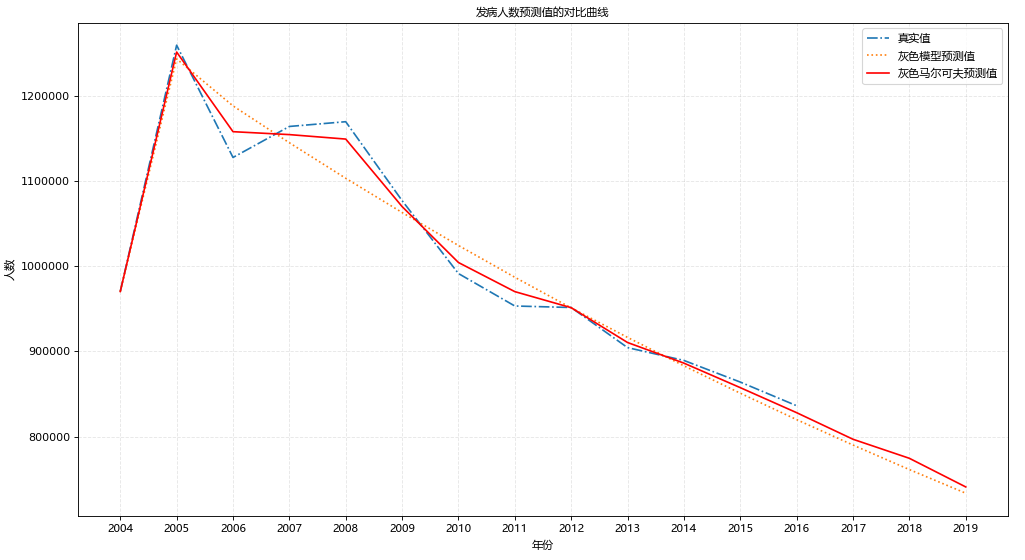
\includegraphics[width=\textwidth]{figures/f.png}
	\caption{发病人数预测对比曲线图}\label{afd}
\end{figure}


	  同理,计算2004-2016年死亡人数预测值得到灰度预测解如下:
	  \begin{gather}
	  	  \widehat{X}(k+1)=-92315e^{-ak}+93750,k=1,2,\cdots,16
	  \end{gather}

	  

	  其误差状态区间如表~\ref{ss}~所示:
	    \begin{table}[H]
	  	\centering\caption{死亡数状态区间划分}\label{ss}
	  	\begin{tabular}{cccc}
	  		\toprule[1.5pt]
	  		\multicolumn{1}{m{2cm}}{\centering 状态}
	  		& \multicolumn{1}{m{3cm}}{\centering $E_{1}$}
	  		& \multicolumn{1}{m{3cm}}{\centering $E_{2}$}
	  		& \multicolumn{1}{m{3cm}}{\centering $E_{3}$}
	  		\\
	  		\midrule[0.5pt]
	  		残差区间 &  $[-684,-228]$  &$(-228,228]$ & $(228,684]$   \\ 
	  		\bottomrule[1.5pt]	
	  	\end{tabular}
	  \end{table}
	  
	  将死亡人数预测值归类于误差区间如表~\ref{sss}~所示:
	  \begin{table}[H]
	  	\centering\caption{死亡人数误差状态区间}\label{sss}
	  	\begin{tabular}{cccccccccccccc}
	  		\toprule[1.5pt]
	  		\multicolumn{1}{m{2cm}}{\centering 年份}
	  		& \multicolumn{1}{m{.7cm}}{\centering 2004}
	  		&\multicolumn{1}{m{.7cm}}{\centering 2005}
	  		& \multicolumn{1}{m{.7cm}}{\centering 2006}
	  		& \multicolumn{1}{m{.7cm}}{\centering 2007}
	  		& \multicolumn{1}{m{.7cm}}{\centering 2008}
	  		& \multicolumn{1}{m{.7cm}}{\centering 2009}
	  		& \multicolumn{1}{m{.7cm}}{\centering 2010}
	  		& \multicolumn{1}{m{.7cm}}{\centering 2011}
	  		& \multicolumn{1}{m{.7cm}}{\centering 2012}
	  		& \multicolumn{1}{m{.7cm}}{\centering 2013}
	  		& \multicolumn{1}{m{.7cm}}{\centering 2014}
	  		& \multicolumn{1}{m{.7cm}}{\centering 2015}
	  		& \multicolumn{1}{m{.7cm}}{\centering 2016}
	  		\\
	  		\midrule[0.5pt]
	  		状态区间 &  $E_{2}$  &$E_{2}$ & $E_{2}$&$E_{3}$ &$E_{1}$ &$E_{3}$&$E_{2}$&$E_{2}$&$E_{2}$&$E_{2}$&$E_{1}$&$E_{2}$&$E_{2}$  \\ 
	  		\bottomrule[1.5pt]	
	  	\end{tabular}
	  \end{table}
	   求得初始状态概率向量$t_{0}'$,转移矩阵$P'$为:
	  \begin{gather}
\begin{matrix}
t_{0}'=[2/13,9/13,2/13]\\ 
\\ 
P'=\left(\begin{array}{lll} 0 & 1/2 & 1/2\\ 1/8 & 3/4 & 1/8 \\1/2 & 1/2 & 0\end{array}\right)
\end{matrix}
	  \end{gather}
	  
       得到由灰色预测与马尔科夫校正后预测解如图~\ref{asf}~所示:
     \begin{figure}[H]
	    \centering
     	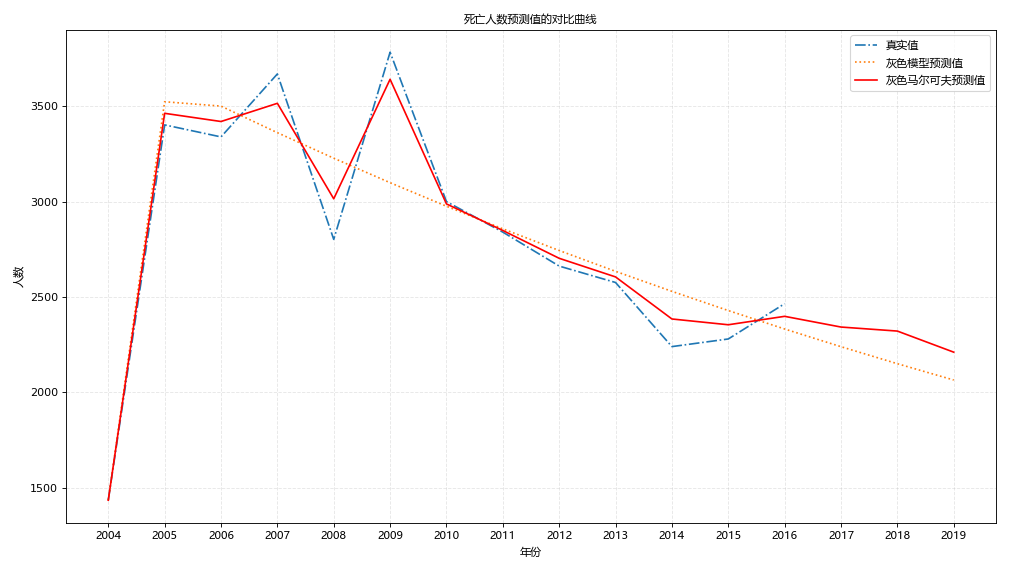
\includegraphics[width=\textwidth]{figures/s.png}
     	\caption{死亡人数预测对比曲线图}\label{asf}
     \end{figure}
 
   \subsection{结果分析}


	根据灰色马尔可夫模型预估出$ 2019$ 年全国感染该疾病的发病人数为 $7.4096\times  10^{5}$,死亡人数为 $2.211\times  10^{3}
	$。由图~\ref{afd}~和图~\ref{asf}~中的预测解曲线直观对比可知,由马尔科夫模型校正后的预测值相较于普通灰色预测值与实际值的\textbf{拟合度更高},波动性一致,且灰色模型预测值是一条相对平滑的曲线,不能反应实际值的波动。两种模型预测指标如表~\ref{jjj}~所示:

 \begin{table}[H]
	\centering\caption{预测结果检验}\label{jjj}
	\begin{tabular}{cccc}
		\toprule[1.5pt]
		\multicolumn{1}{m{6cm}}{\centering 检验参数}
		& \multicolumn{1}{m{2cm}}{\centering RMSE}
		& \multicolumn{1}{m{2cm}}{\centering MAPE}
		& \multicolumn{1}{m{2cm}}{\centering NSE}
		\\
			\midrule[0.5pt]	
	    传统灰色预测数值(患病数) &   30040.04 &  0.0213 & 0.9455\\ 
		灰色马尔科夫预测数值(患病数)&  12838.64  &  0.0095  &  0.9900 \\ 
		传统灰色预测数值(死亡数) &  265.88   & 0.0628   &0.8178  \\
		灰色马尔科夫预测数值(死亡数) &   101.13 &   0.0273 & 0.9736  \\   
		\bottomrule[1.5pt]	
	\end{tabular}
\end{table} 

从上述的预测结果可以得出:利用灰色马尔科夫模型修正后求出的患病人数与死亡人数的均方根误差值RMSE,其值都小于传统灰色模型预测值RMSE值,表明\textbf{校正后结果可靠性更高}。且修正后模型MPAE值较于传统模型更接近$0$,NSE值更接近 $1$,说明改进后的灰色马尔科夫模型的\textbf{拟合程度更高},\textbf{预测效果更好},适用于传染病发病数和死亡数的短期预测。


	  
	  \section{问题二模型的建立与求解}
	  \subsection{问题描述与分析}

	 问题二本质是一个预测与综合评价问题,题目要求结合不同地区和职业分类统计的数据,预测2019年传染病防控排名前3位的重点区域和重点人群。首先将附件中不同地区与不同职业的发病人数、死亡人数数据,带入问题一的\textbf{灰色马尔科夫模型}中。预测出2019年各省与各职业的发病人数、死亡人数,并计算出每个地区和每种职业对应的发病人数\textbf{增长率、死亡人数增长率和死亡率}。并将上述五个指标带入\textbf{TOPSIS综合评价模型},分别选取排序前三位的省市和人群作为重点防控区域和人群。其问题二思维流程图如图~\ref{lctcc}~所示:
	 \begin{figure}[H]
	 	\centering
	 	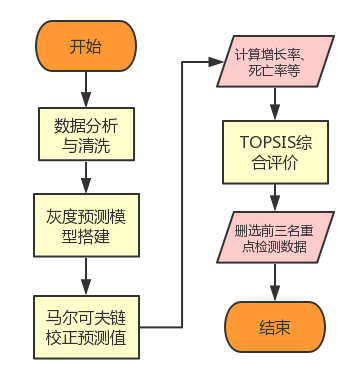
\includegraphics[width=.5\textwidth]{figures/lctcc.png}
	 	\caption{问题二思维流程图}\label{lctcc}
	 \end{figure}
	  \subsection{模型的建立}
	  根据各年数据的不同对第一问的灰色马尔可夫模型进行修正,得:
	  \begin{gather}
\left\{\begin{matrix}
\overline{x}(k) =\widehat{x}(k)-\eta\\
\widehat{X}(k+1)=[X^{(0)}(1)-\frac{u}{a}]e^{-ak}+\frac{u}{a},k=1,2,\cdots,6\\ 
\eta =\begin{bmatrix}
p_{E1} & p_{E2} & p_{E3}
\end{bmatrix} \cdot \begin{bmatrix}
\overline{E}_{1} & \overline{E}_{2} & \overline{E}_{3}
\end{bmatrix}^{T}
\end{matrix}\right.
	  \end{gather}
	 式中:第$k$年的患病或死亡人数据修正后预测值为$\overline{x}(k)$,$\widehat{x}(k)$为传统GM(1,1)的预测值,$\eta$为第$k$年GM(1,1)的误差期望值。
	     \subsubsection{预测评价指标计算}
	     
	     
	     
	  将附件中$20$个职业2004年,2007年,2010年,2013年和2016年的患病人数数据$X_{i}=[x_{i1},x_{i2},x_{i3},x_{i4},x_{i5}](i=1,2,\cdots,20)$,带入后,得到预测结果:
     \begin{gather*}
      X_{i}=[x_{i1},x_{i2},x_{i3},x_{i4},x_{i5},x_{i6}](i=1,2,\cdots,20)
     \end{gather*}
     
     同理,将死亡人数数据$X_{i}'=[x_{i1}',x_{i2}',x_{i3}',x_{i4}',x_{i5}'](i=1,2,\cdots,20)$带入得到预测结果$X_{i}'=[x_{i1}',x_{i2}',x_{i3}',x_{i4}',x_{i5}',x_{i6}'](i=1,2,\cdots,20)$。


     则预测中2019年发病人数增长率$ \delta_{i}$、死亡人数增长率 $ \delta _{i}'$和患病人口死亡率$\eta_{i}$分别为:
      \begin{gather}
      \left\{\begin{matrix}
      \delta _{i}=\frac{x_{i6}-x_{i5}}{x_{i5}} \times 100\%\\ 
      \delta '_{i} =\frac{x_{i6}'-x_{i5}'}{x_{i5}'} \times 100\%\\ 
      \eta_{i} =\frac{x_{i6}'}{x_{i6}} \times 100\%
      \end{matrix}\right.
      \end{gather}
      得到各个人群的决策属性向量:
      \begin{gather*}
      d_{i}=[x_{i6},x_{i6}', \delta_{i} , \delta _{i}',\eta_{i} ]
      \end{gather*}
      
      同理,将全国各省即直辖市各年患病人口与死亡人口数据带入模型可得各个地区的决策属性向量$d_{i}'(i=1,2,\cdots,31)$。
    \subsubsection{TOPSIS法}
    设职业多属性决策矩阵$A=(a_{ij})_{20 \times 5}$可表示为:
     \begin{gather*}
  A= [d_{1}^{T},d_{2}^{T},\cdot,,d_{20}^{T}]^{T}
    \end{gather*}
    将$A$标准化可得规范化决策矩阵$B=(b_{ij})_{20 \times 5}$,其中:
     \begin{gather*}
   b_{ij}=a_{ij}/\sqrt{\sum_{i=1}^{20}a_{ij}^{2}},i=1,2,\cdots,20;j=1,2,\cdots,5
    \end{gather*}
    
    假定\textbf{患病人数和死亡人数增长率高的区域更需要重点防控},构造权重向量:
     \begin{gather}
     W=[0.15,0.3,0.15,0.3,0.1]
    \end{gather}
    即可求得加权规范矩阵为$C=(c_{ij})_{20 \times 5}$、正理想解$C^{*}=[c_{1}^{*},c_{2}^{*},c_{3}^{*},c_{4}^{*},c_{5}^{*}]$、负理想解$C^{0}=[c_{1}^{0},c_{2}^{0},c_{3}^{0},c_{4}^{0},c_{5}^{0}]$,其中:
     \begin{gather*}
     \begin{matrix}
     c_{ij}=w_{j} \cdot b_{ij} ,i=1,2,\cdots,20;j=1,2,\cdots,5\\
c_{j}^{*}=\underset{i}{max}(c_{ij}) ,j=1,2,\cdots,5\\
c_{j}^{0}=\underset{i}{min}(c_{ij}) ,j=1,2,\cdots,5
     \end{matrix}
    \end{gather*}
    
    计算各职业属性决策向量到正理想解和负理想解的距离。备选职业属性决策向量$d_{i}$到正理想解的距离为与到负理想解的距离为:
    \begin{gather*}
    s_{j}^{*}=\sqrt{\sum_{j=1}^{n}(c_{ij}-c_{j}^*)^{2}},i=1,2,\cdots,20\\
    s_{j}^{0}=\sqrt{\sum_{j=1}^{n}(c_{ij}-c_{j}^{0})^{2}},i=1,2,\cdots,20
    \end{gather*}
    计算各方案的综合评价指数:
    \begin{gather}
    f_{i}^{*}=s_{j}^{0}/(s_{j}^{0}+s_{j}^{*}),i=1,2,\cdots,20
    \end{gather}

    按$f_{i}^{*}$由大到小排列求得重点防控人群次序。同理将各地区决策向量$d_{i}'(i=1,2,\cdots,31)$带入TOPSIS模型可得重点防控地区次序即可。

    \subsection{模型的求解}

 
         将各职业的患病人数与死亡人数的数据,带入灰度马尔科夫模型得到预测值如表~\ref{zhiye1}~、~\ref{zhiye2}~所示:
    \begin{table}[H]
    	\centering\caption{各职业发病数预测结果}\label{zhiye1}
    	\begin{tabular}{ccccccc}
    		\toprule[1.5pt]
    		\multicolumn{1}{m{2cm}}{\centering 职业}
    		& \multicolumn{1}{m{1.8cm}}{\centering 2004}
    		& \multicolumn{1}{m{1.8cm}}{\centering 2007}
    		& \multicolumn{1}{m{1.8cm}}{\centering 2010}
    		& \multicolumn{1}{m{1.8cm}}{\centering 2013}
    		& \multicolumn{1}{m{1.8cm}}{\centering 2016}
    		& \multicolumn{1}{m{1.8cm}}{\centering 2019}
    		\\
    		\midrule[0.5pt]	
    		幼托儿童 &   2239 & 1416.433 &	552.277 &	218.444& 	86.402& 	34.175 \\ 
    		散居儿童&  6179  &  3759.599&	2454.325	&1638.953&	1094.463&730.862\\ 
    		学生 &  61578  & 65186.262 &	50766.106 &	40071.014 &	31629.098 	&24965.674  \\
    		$\cdots$ &  $\cdots$ &  $\cdots$&  $\cdots$&  $\cdots$&  $\cdots$&  $\cdots$   \\   
    		家政、家务 & 54916& 67490.081&78063.992&91181.696&106503.671 &124400.317 \\ 
    		其他 & 34028 &54221.751 &	40402.927 &	29919.473 &	22156.188&16407.263  \\
    		\bottomrule[1.5pt]	
    	\end{tabular}
    \end{table}

    \begin{table}[H]
    	\centering\caption{各职业死亡数预测结果}\label{zhiye2}
    	\begin{tabular}{ccccccc}
    		\toprule[1.5pt]
    		\multicolumn{1}{m{2cm}}{\centering 职业}
    		& \multicolumn{1}{m{1.8cm}}{\centering 2004}
    		& \multicolumn{1}{m{1.8cm}}{\centering 2007}
    		& \multicolumn{1}{m{1.8cm}}{\centering 2010}
    		& \multicolumn{1}{m{1.8cm}}{\centering 2013}
    		& \multicolumn{1}{m{1.8cm}}{\centering 2016}
    		& \multicolumn{1}{m{1.8cm}}{\centering 2019}
    		\\
    		\midrule[0.5pt]	
    		幼托儿童 &  2&1.858&	1.012&0.571&	0.323&0.182
    		\\ 
    		散居儿童& 9	 &14.193&	10.118&	7.270 &	5.223&3.753
    		\\ 
    		学生 & 22 &	38.123 &30.824 &24.931 &20.164& 16.309   \\
    		$\cdots$ &  $\cdots$ &  $\cdots$&  $\cdots$&  $\cdots$&  $\cdots$&  $\cdots$   \\   
    		家政、家务 &  133&	244.727 &	271.116 &	301.405 &	335.077 &	372.512 \\ 
    		其他 &  46&	143.799 &	101.315 &	70.427 &	48.956 	&34.031 \\
    		\bottomrule[1.5pt]	
    	\end{tabular}
    \end{table}
    
    计算出正理想解与负理想解分别为:
\begin{gather*}
\begin{matrix}
C^{0}=[0.0066,0.0048,0.0653,0.0261,0.0331]\\
C^{*}=[-0.1856,-0.1847,-0.0809,-0.1163,-0.0929]
\end{matrix}
\end{gather*}
    即求得$20$种职业综合评价指数如图~\ref{oc}~所示:
    \begin{figure}[H]
    	\centering
    	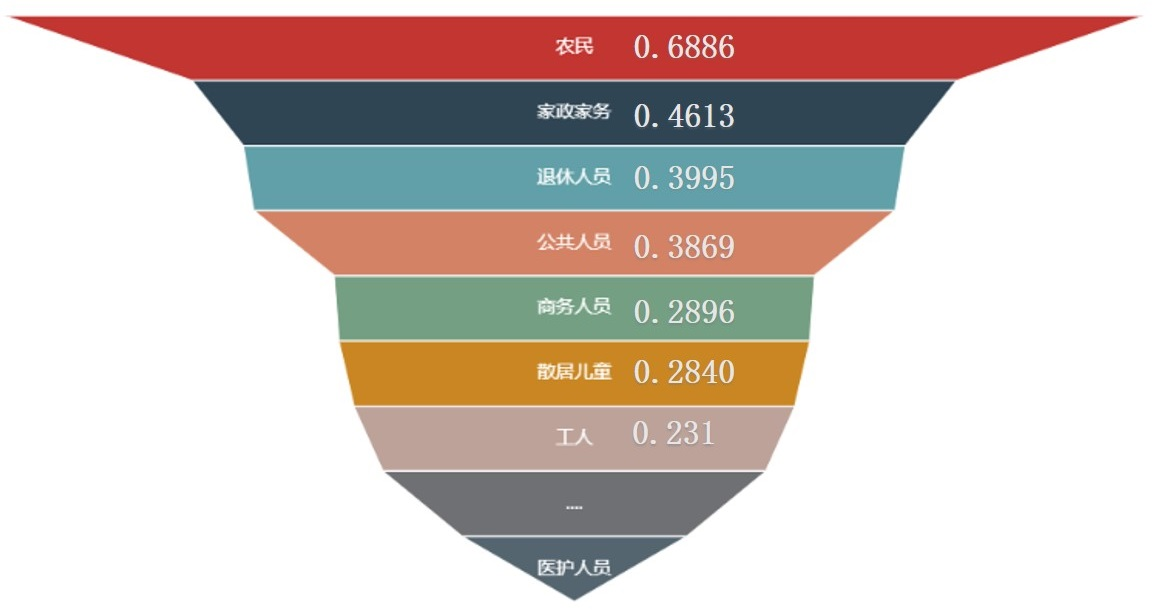
\includegraphics[width=\textwidth]{figures/oc.png}
    	\caption{人群综合评价指数}\label{oc}
    \end{figure}
	由图~\ref{oc}~可知防控排名前$3$位的\textbf{职业分别为农民、家政家务和退休人员}。


    
   同理,将各地区患病人数与死亡人数预测值带入模型,得到2019年预测值见附件。计算出正理想解与负理想解$
   C^{*}$、$C^{0}$。即可求得$31$个地区综合评价指数如图~\ref{area}~所示:
   \begin{figure}[H]
   	\centering
   	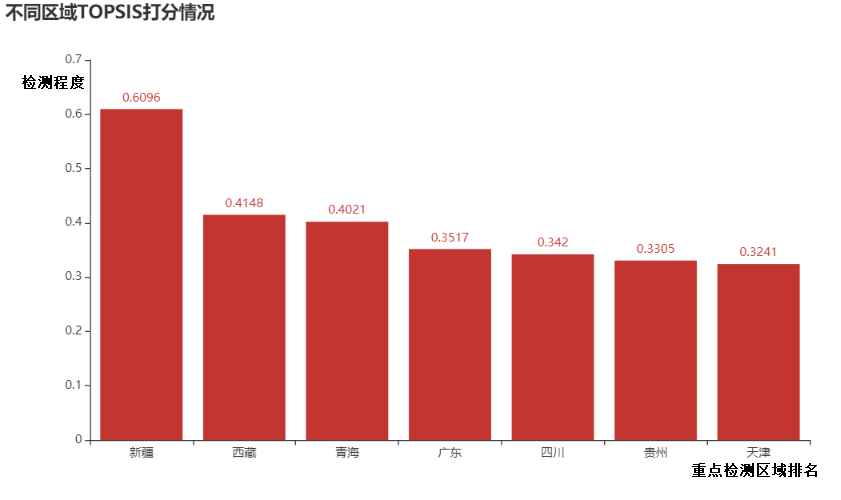
\includegraphics[width=\textwidth]{figures/area.png}
   	\caption{地区综合评价指数}\label{area}
   \end{figure}
   由图~\ref{area}~可知防控排名前$3$位的\textbf{地区分别为新疆,西藏和青海}。


\subsection{结果分析}
农民、家政家务和退休人员的发病人数、死亡人数灰色马尔科夫预测曲线如下图所示:
	\begin{figure}[H]
	\begin{minipage}[t]{0.5\linewidth}
		%并排插图时,线宽很重要,自己慢慢试,俩张图就不要超过0.5,三张图不要超过0.33之类的,自己看着办
		\centering
		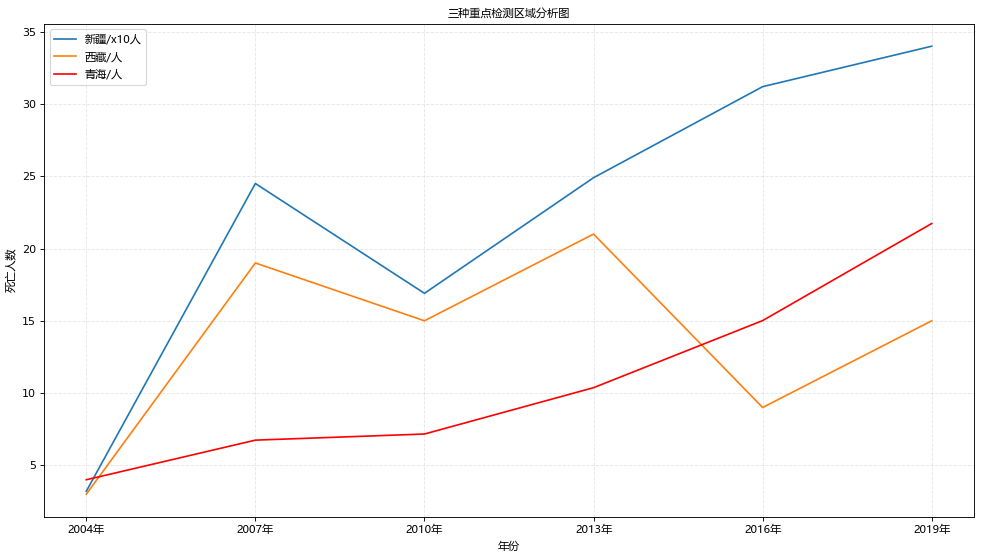
\includegraphics[width=\textwidth]{figures/Figure_6.png}
		\caption{职业前三每年发病人数}\label{sanrenf}
	\end{minipage}
	\hfill%分栏的意思吧
	\begin{minipage}[t]{0.5\linewidth}
		\centering
		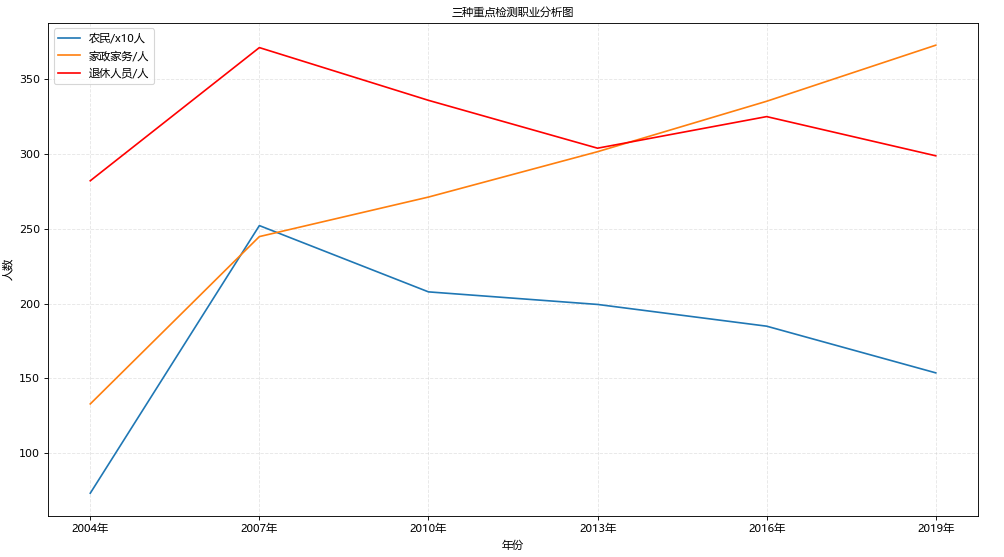
\includegraphics[width=\textwidth]{figures/sannrens.png}
		\caption{职业前三每年死亡人数}\label{sannrens}
	\end{minipage}
\end{figure}

由图~\ref{sanrenf}~和图~\ref{sannrens}~可知家政家务从业人员发病人数和死亡人数都处于上升趋势,且\textbf{上升率较高},属于重点防控人群。而农民发病人数和死亡人数都虽处于下降趋势但其\textbf{患病人口基数较大}导致其综合评价指数较高,属于重点防控人群。而退休人口发病人数和死亡人数的增长率和基数都不大,但其发病后死亡较高,也属于重点防控人群。

新疆,西藏和青海的灰色马尔科夫预测曲线如下图所示:
	\begin{figure}[H]
	\begin{minipage}[t]{0.5\linewidth}
		%并排插图时,线宽很重要,自己慢慢试,俩张图就不要超过0.5,三张图不要超过0.33之类的,自己看着办
		\centering
		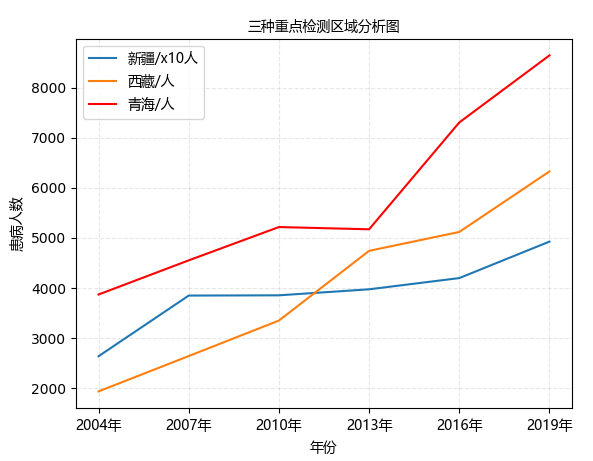
\includegraphics[width=\textwidth]{figures/Figure_5.png}
		\caption{前三省份每年发病人数}\label{Figure_5}
	\end{minipage}
	\hfill%分栏的意思吧
	\begin{minipage}[t]{0.5\linewidth}
		\centering
		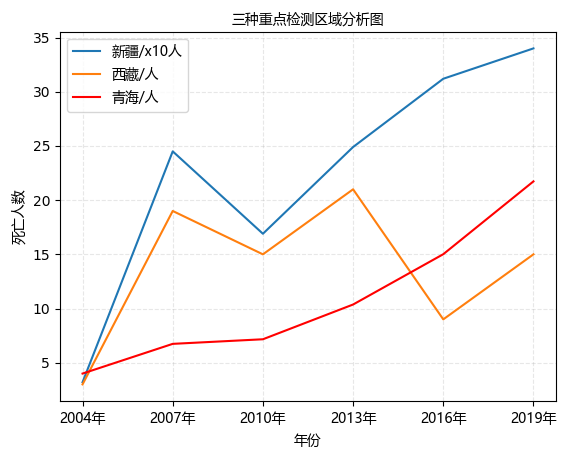
\includegraphics[width=\textwidth]{figures/Figure_1.png}
		\caption{前三省份每年死亡人数}\label{Figure_6}
	\end{minipage}
\end{figure}
由图~\ref{Figure_5}~和图~\ref{Figure_6}~可知新疆,西藏和青海的\textbf{发病人数和死亡人数都处于整体上升趋势},尤其是新疆还有相对于其它二者较大的患病人口基数,都属于重点防控区域。
。

     	\section{问题三模型的建立与求解}
     \subsection{问题描述与分析}


    问题三本质是多元回归预测问题,题目要求结合地区经济发展的相关公开数据,建立该传染病与经济发展的数学模型。首先收集$31$个省市2004年,2007年,2010年,2013年和2016年的经济发展数据。通过灰色关联度分析得到经济指标中与患病人数和死亡人数灰色关联度排名前三的是\textbf{人均GDP}、\textbf{居民消费水平}和\textbf{一般预算收入}。再基于\textbf{SMO-SVR回归}得出经济指标分别对于患病人数和死亡人数的回归分析模型。其经济指标的部分数据如下表:

             \begin{table}[H]
    	\centering\caption{各省每年经济指标的数据}\label{s2ss}
    	\begin{tabular}{cccccc}
    		\toprule[1.5pt]
    		\multicolumn{1}{m{1.8cm}}{\centering 时域
    		}
    		& \multicolumn{1}{m{1.8cm}}{\centering 人均GDP}
    		& \multicolumn{1}{m{1.8cm}}{\centering 地区生产总值}
    		& \multicolumn{1}{m{1.8cm}}{\centering 居民消费水平
    		}
    		& \multicolumn{1}{m{1.8cm}}{\centering 一般预算收入
    		}
      		& \multicolumn{1}{m{1.8cm}}{\centering 一般预算支出
      		}
    		  
    		\\
    		\midrule[0.5pt]	
    		北京2004 & 37058 &6060&12405&744&898
    		\\ 
    		北京2007 & 58204&9846&18911&1492&1649\\
    		北京2010 &73856 &14113&25015&2353&2717\\
    		北京2013 & 94648&19155&33337&3661&4242\\
    		北京2016 & 118198&25669&48883&5081&6406\\
    		天津2004 &31165 &3110&8765&246&375\\
    		$\cdots$ &$\cdots$ &$\cdots$&$\cdots$&$\cdots$&$\cdots$\\
    		新疆2016 &24543 &4245&14424&2403&5241\\
    		\bottomrule[1.5pt]	
    	\end{tabular}
    \end{table}

   
     \subsection{模型的建立}
     	\subsubsection{灰色关联分析}
     由于考虑到患病数与死亡数受多个经济因素的影响,我们采取灰色关联分析来分析各个因素对于结果的影响程度,根据分析结果来选择回归模型中的自变量。灰色关联分析是指对一个系统发展变化态势的定量描述和比较的方法,其基本思想是通过确定参考数据列和若干个比较数据列的几何形状相似程度来判断其联系是否紧密,它反映了曲线间的关联程度。首先对每个特征确定分析数列并做归一化,再进行关联系数,其公式如下:
     
     \begin{gather}
     \xi _{i}\left ( k \right )=\frac{min_{i} min_{k}\Delta _{i}(k)+\rho max_{i} max_{k}\Delta _{i}(k)}{\Delta _{i}(k)+\rho max_{i} max_{k}\Delta _{i}(k)}
     \end{gather}
     
     
     式中记$\Delta _{i}(k)=|y(k)-x_{i}(k)|$,$\rho \in (0,\infty )$称为分辨系数。$\rho $越小,分辨力越大,一般$\rho $的取值区间为(0,1),具体取值可视情况而定。
 \begin{figure}[H]
 	\centering
 	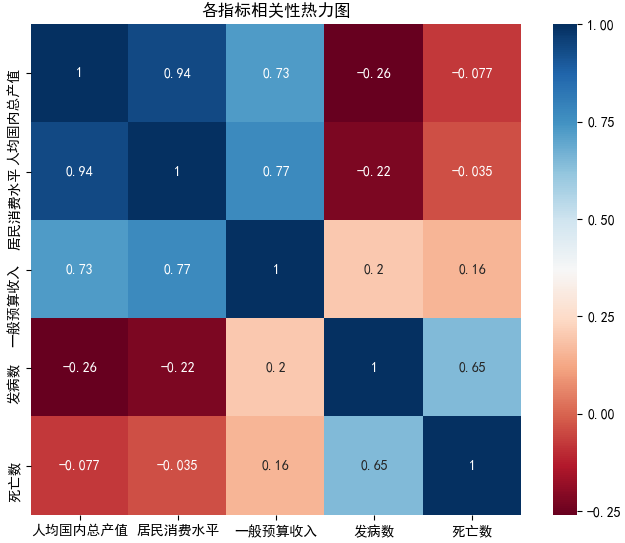
\includegraphics[width=.7\textwidth]{figures/Figure_8.png}
 	\caption{相关系数矩阵热力图}\label{re}
 \end{figure}
     	
     	通过灰色关联分析得到\textbf{人均GDP,居民消费水平,一般预算收入}三个特征的$\rho $分别为0.917019、0.892481、0.833659。分辨力均较好,即都与传染病相关联。因此在回归模型中同时考虑3种经济因素。

     
     
     \subsection{SMO-SVR模型}   
     	由于灰色马尔可夫模型只支持时间序列上的短期预测,为建立经济与传染病之间的数学模型,本组改用支持向量回归对两者进行拟合。SVR的基本思想是寻找一个最优分类而使得所有训练样本离该最优分类面的误差最小。参考Kate Childs等人的文章\cite{bib:7},建立出三维经济决策向量与传染病之间的SVR模型。
     为减小算法复杂度,使用序列最小优化算法(SMO)作为样本训练算法,进而建立了序列最小优化支持向量回归模型(SMO-SVR)。\cite{bib:8}
          \begin{gather}
     f(x)=\sum_{i=1}^{n}\left(\alpha_{i}-\alpha_{i}^{*}\right)<x_{i}, x>+b
     \end{gather}\label{svr}
     
     \subsection{模型的求解与分析}
     通过建立的SMO-SVR模型,首先以各省各年的人均GDP,居民消费水平,一般预算收入标准化后的经济作为模型的输入变量,然后分别对发病数、死亡数进行序列最小优化支持向量回归预测,最终得到预测结果:
     
     	\begin{figure}[H]
     	\begin{minipage}[t]{0.5\linewidth}
     		%并排插图时,线宽很重要,自己慢慢试,俩张图就不要超过0.5,三张图不要超过0.33之类的,自己看着办
     	\centering
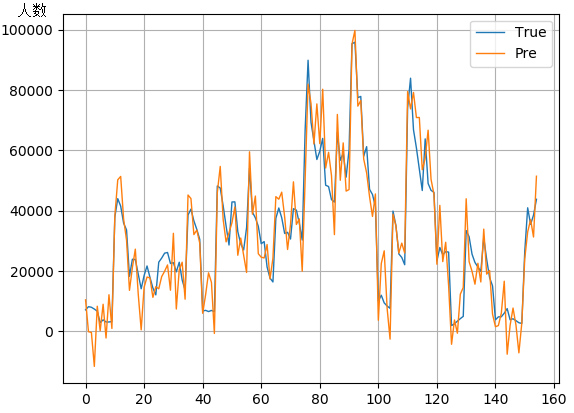
\includegraphics[width=\textwidth]{figures/Figure_9.png}
\caption{发病人数预测结果}\label{Figure_9}
     	\end{minipage}
     	\hfill%分栏的意思吧
     	\begin{minipage}[t]{0.5\linewidth}
     	\centering
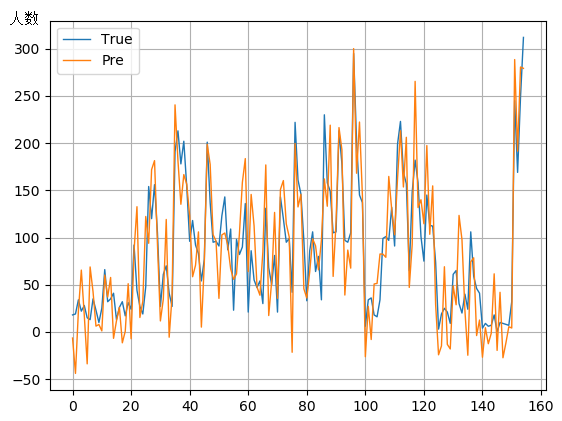
\includegraphics[width=\textwidth]{figures/Figure_10.png}
\caption{死亡人数预测结果}\label{Figure_10}
     	\end{minipage}
     \end{figure}
         \begin{table}[H]
     	\centering\caption{各职业发病数预测结果}\label{zhiye1}
     	\begin{tabular}{cccc}
     		\toprule[1.5pt]
     		\multicolumn{1}{m{2cm}}{\centering 检验参数}
     		& \multicolumn{1}{m{1.8cm}}{\centering RMSE}
     		& \multicolumn{1}{m{1.8cm}}{\centering MAPE}
     		& \multicolumn{1}{m{1.8cm}}{\centering NSE}
     		\\
     		\midrule[0.5pt]	
     		经济与发病 &  $7.7523\times10^{3}$&$0.0386$&$0.878$
     		\\ 
     		经济与死亡 &  $449.273$&$0.0154$&$0.943$\\
     		\bottomrule[1.5pt]	
     	\end{tabular}
     \end{table}
     

     
    \section{问题四:写给卫生健康委员会相关部门的一封公开信}
    \textbf{致卫生健康委员会相关部门的一封信}:
    ~\\
    
    随着全球化的进程,人类活动范围日益扩大,人群流动频繁,传染病可在大范围内迅速传播,是对人类社会存在威胁的公共卫生问题。传染病的防治与人民的身体健康和生命安全有着密切的关系,关系着经济社会发展和国家安全稳定。近十几年来,我国先后爆发了非典型性肺炎(SARS),高致病性禽流感H5N1,甲型H1N1流感等突发传染病疫情,均对生命健康和社会生活造成了重大影响。艾滋病、肺结核病等重大传染病防治形势依然严峻,防治工作任务繁重。如何遏制传染病爆发,缓解传染病流行,是当今社会面临的紧迫问题。为了提高传染病疫情和突发公共卫生事件报告的质量和时效,加强对全国传染病感染病人的诊断、治疗和监督管理,建立完善的全国卫生监管机制是目前最为紧急的事情。
    
    在疾病控制实际工作中,疾病的发病与流行趋势分析是极其重要的一环,科学、准确的分析能对卫生行政部分制定疾病预防与控制策略产生重要的影响,传染病早期预警将大大降低传染病的社会经济危害。卫生部门应通过对疫情的动态分析及时指定出防治的对策和策略,以控制并逐渐消灭各类传染病,提早全国人民的生活及健康水平。构建预测模型从早期探测到传染病的爆发并及时预警,采取应对措施,是目前传染病防控的重要手段,具有重要的实际意义。因此我们建立了某传染病指标模型,在分析传染病的变化趋势和预测方面有很大的理论和现实意义,并向贵部门提出相关建议。
    
    我们基于灰色预测模型,利用马尔可夫模型对其进行改进,结合2004-2016年全国的发病数和死亡数,预测得到了2019年全国感染该疾病的发病人数和死亡人数。通过统计和分析2004-2016年全国各地区及不同职业分类的发病数和死亡数,建立了传染病传播模型,结合原有模型的预测结果,我们引入了TOPSIS模型,根据有限个评价对象与理想化目标的接近程度进行排序的方法,对现有的对象进行相对优劣的评价。得到了不同地区和不同人群的综合评价指数。对其进行排序后,得到了排名前三的重点防控区域和职业分类,这对相应地区的卫生部门制定策略计划具有重要的参考价值。并结合地区的经济发展情况,建立了传染病与经济发展相关的数学模型。
    
    伴随着经济的快速发展,全国范围的医疗水平有显著提高,人们的生活环境和卫生水平也得到明显改善,现传染病的传播速率较往年已有减缓趋势。但经济的增长也使流动人口迅速增加,导致了传染病的传播范围扩大和疫情控制的难度提高。 
    
    因此针对以上情况我们向有关部门提出以下建议:
    \begin{itemize}                                             
    	\item [(1)] 要建立完善的公共卫生监管数据库,对包括偏远地区在内的区域要尽快地普及,建立监管机制,当传染病疫情出现预警或发生时,应及时统计并分析疫情的相关信息和数据,制定相应的防治对策。
    	\item[(2)]努力提高全国地医疗水平,加大对偏远落后地区地医疗投入力度,提高对他们的技术支持,对重点防控区域和人群要有针对性地实施政策。
    	\item [(3)]加大对群众卫生健康知识的宣传,提高群众们的防范意识。
    	\item [(4)]对于流动人口多、人口基数大的城市应重点防控,增加各类流行传染病药物库存。
    	\item [(5)]更好地完善和改进医疗制度,缓解解决百姓中“看病难”、“看病贵”等疑难问题,落实医疗改革成果,提升医疗卫生服务能力,结合现代化智能网络技术,开发与建立线上远程医疗平台。	
    \end{itemize}
	以上建议仅供参考,不足之处请予以批评指正。


	\section{模型的评价}
	\subsection{模型的优点}
		\begin{itemize}                                             

		\item [(1)] 利用马尔可夫模型改进后的灰度预测值与实际值拟合度更高,波动性保持一致,预测的效果更好
		\item [(2)] 针对支持向量回归参数选取,利用灰色关联度筛选合适指标,相较于主观选取指标具有客观性、严谨性。
		
	\end{itemize}
	\subsection{模型的缺点}
	
	
	\subsection{模型改进}
	

 
	\newpage	%换页符
	%%参考文献
	%\begin{thebibliography}{9}%宽度9
	% \setlength{\itemsep}{-2mm}
	\nocite{*}		%排版未引用的参考文献
%\bibliography{wenxian.bib}
%	%参考文献添加到wenxian.bib里,再引用
%	
\begin{thebibliography}{9}%宽度9
	\bibitem{bib:one}Saad Ahmed Javed,Sifeng Liu. Correction to: Predicting the research output/growth of selected countries: application of Even GM (1, 1) and NDGM models[J]. Scientometrics,2019,120(3).
	\bibitem{bib:2}李立欣,文海东,许健开.基于灰色马尔可夫模型的能源消耗预测[J].中国科技信息,2018(15):74-75.	
	\bibitem{bib:3}Yawen Wang,Zhongzhou Shen,Yu Jiang. Analyzing maternal mortality rate in rural China by Grey-Markov model[J]. Medicine,2019,98(6).
	\bibitem{bib:4}Saad Ahmed Javed,Sifeng Liu. Correction to: Predicting the research output/growth of selected countries: application of Even GM (1, 1) and NDGM models[J]. Scientometrics,2019,120(3).
	\bibitem{bib:5}成枢,周龙飞,高秀明.基于灰色关联GM(1,N)-Markov修正模型的应用[J].勘察科学技术,2019(03):43-48.
	\bibitem{bib:6}刘永阔,谢春丽,于竹君,凌霜寒.基于GM(1,1)模型与灰色马尔可夫GM(1,1)模型的核动力装置趋势预测方法研究[J].原子能科学技术,2011,45(09):1075-1079.
	\bibitem{bib:7}Kate Childs,Christopher Davis,Mary Cannon,Sarah Montague,Ana Filipe,Lily Tong,Peter Simmonds,Donald Smith,Emma C. Thomson,Geoff Dusheiko,Kosh Agarwal. Suboptimal SVR rates in African patients with atypical Genotype 1 subtypes: implications for global elimination of Hepatitis C[J]. Journal of Hepatology,2019.
	\bibitem{bib:8}Yuyan Cao. Failure Prognosis for Electro-Mechanical Actuators Based on Improved SMO-SVR Method[A]. 中国航空学会制导、导航与控制分会、飞行器控制一体化技术重点实验室、IEEE控制系统协会南京分会.Proceedings of 2016 IEEE Chinese Guidance, Navigation and Control Conference (IEEE CGNCC2016)[C].2016:6.
\end{thebibliography}

	\newpage
	%附录
	\appendix %%附录

\section{代码}
\subsection{灰色马尔可夫模型--matlab源代码}
\begin{lstlisting}[language=matlab]
x = [970279 1259308 1127571 1163959 1169540 1076938 991350 953275 951508 904434 889381 864015 836236];

%二次拟合预测GM(1,1)模型
sizexd2 = size(x,2);
%求数组长度

k=0;
for y1=x
k=k+1;
if k>1
x1(k)=x1(k-1)+x(k);
%累加生成
z1(k-1)=-0.5*(x1(k)+x1(k-1));   
%z1维数减1,用于计算B
yn1(k-1)=x(k);
else
x1(k)=x(k);
end
end
%x1,z1,k,yn1

sizez1=size(z1,2);
%size(yn1);
z2 = z1';
z3 = ones(1,sizez1)';

YN = yn1';   %转置
%YN

B=[z2 z3];
au0=inv(B'*B)*B'*YN;
au = au0';
%B,au0,au

afor = au(1);
ufor = au(2);
ua = au(2)./au(1);
%afor,ufor,ua 
%输出预测的  a u 和 u/a的值

constant1 = x(1)-ua;
afor1 = -afor;
x1t1 = 'x1(t+1)';
estr = 'exp';
tstr = 't';
leftbra = '(';
rightbra = ')';
%constant1,afor1,x1t1,estr,tstr,leftbra,rightbra

strcat(x1t1,'=',num2str(constant1),estr,leftbra,num2str(afor1),tstr,rightbra,'+',leftbra,num2str(ua),rightbra)
%输出时间响应方程

%******************************************************
%二次拟合

k2 = 0;
for y2 = x1
k2 = k2 + 1;
if k2 > k  
else
ze1(k2) = exp(-(k2-1)*afor);  
end
end
%ze1

sizeze1 = size(ze1,2);
z4 = ones(1,sizeze1)';
G=[ze1' z4];
X1 = x1';
au20=inv(G'*G)*G'*X1;
au2 = au20';
%z4,X1,G,au20

Aval = au2(1);
Bval = au2(2);
%Aval,Bval
%输出预测的  A,B的值

strcat(x1t1,'=',num2str(Aval),estr,leftbra,num2str(afor1),tstr,rightbra,'+',leftbra,num2str(Bval),rightbra)
%输出时间响应方程

nfinal = sizexd2-1 + 3;
%决定预测的步骤数5  这个步骤可以通过函数传入

%nfinal = sizexd2 - 1 + 1;
%预测的步骤数 1

for  k3=1:nfinal
x3fcast(k3) = constant1*exp(afor1*k3)+ua;
end
%x3fcast
%一次拟合累加值

for  k31=nfinal:-1:0
if k31>1
x31fcast(k31+1) = x3fcast(k31)-x3fcast(k31-1);
else
if k31>0
x31fcast(k31+1) = x3fcast(k31)-x(1);
else
x31fcast(k31+1) = x(1);
end
end

end
x31fcast
%一次拟合预测值


for  k4=1:nfinal
x4fcast(k4) = Aval*exp(afor1*k4)+Bval;
end
%x4fcast

for  k41=nfinal:-1:0
if k41>1
x41fcast(k41+1) = x4fcast(k41)-x4fcast(k41-1);
else
if k41>0
x41fcast(k41+1) = x4fcast(k41)-x(1);
else
x41fcast(k41+1) = x(1);
end
end

end
x41fcast,x
%二次拟合预测值

%***精度检验p C************//////////////////////////////////
k5 = 0;
for y5 = x
k5 = k5 + 1;
if k5 > sizexd2  
else
err1(k5) = x(k5) - x41fcast(k5);  
end
end
%err1
%绝对误差


xavg = mean(x);
%xavg
%x平均值

err1avg = mean(err1);
%err1avg
%err1平均值

k5 = 0;
s1total = 0 ;
for y5 = x
k5 = k5 + 1;
if k5 > sizexd2  
else
s1total = s1total + (x(k5) - xavg)^2;  
end
end
s1suqare = s1total ./ sizexd2;
s1sqrt = sqrt(s1suqare);
%s1suqare,s1sqrt
%s1suqare  残差数列x的方差  s1sqrt 为x方差的平方根S1

k5 = 0;
s2total = 0 ;
for y5 = x
k5 = k5 + 1;
if k5 > sizexd2  
else
s2total = s2total + (err1(k5) - err1avg)^2;  
end
end
s2suqare = s2total ./ sizexd2;
%s2suqare   残差数列err1的方差S2

Cval = sqrt(s2suqare ./ s1suqare);
%nnn = 0.6745 * s1sqrt
%Cval  C检验值

k5 = 0;
pnum = 0 ;
for y5 = x
k5 = k5 + 1;
if abs( err1(k5) - err1avg ) < 0.6745 * s1sqrt
pnum = pnum + 1;
%ppp = abs( err1(k5) - err1avg )     
else
end
end
pval = pnum ./ sizexd2;

%p检验值

%arr1 = x41fcast(1:6)
\end{lstlisting}

\subsection{TOPSIS分析--matlab源代码}
\begin{lstlisting}[language=matlab]
function [ output_args ] = TOPSIS(A,W)

%A为决策矩阵,W为权值矩阵,M为正指标所在的列,N为负指标所在的列
[ma,na]=size(A);          %ma为A矩阵的行数,na为A矩阵的列数
for i=1:na
B(:,i)=A(:,i)*W(i);     %按列循环得到[加权标准化矩阵]
end
V1=zeros(1,na);            %初始化正理想解和负理想解
V2=zeros(1,na);
BMAX=max(B);               %取加权标准化矩阵每列的最大值和最小值
BMIN=min(B);               %

for i=1:na
%if i<=size(M,2)        %循环得到理想解和负理想解,注意判断,不然会超个数
V1(i)=BMAX(i);
V2(i)=BMIN(i);
%end
%if i<=size(N,2)
%V1(N(i))=BMIN(N(i));
%V2(N(i))=BMAX(N(i));
%end
end

for i=1:ma                 %按行循环求各方案的贴近度
C1=B(i,:)-V1;
S1(i)=norm(C1);        %S1,S2分别为离正理想点和负理想点的距离,用二阶范数

C2=B(i,:)-V2;
S2(i)=norm(C2);
T(i)=S2(i)/(S1(i)+S2(i));     %T为贴近度
end
C1
C2
output_args=T;
\end{lstlisting}
\subsection{数据可视化--python源代码}
\begin{lstlisting}[language=python]
from example.commons import Faker
from pyecharts import options as opts
from pyecharts.charts import Bar
from pyecharts.globals import ThemeType
# 新疆:0.8096,西藏:0.4148,青海:0.4021,广东:0.3517,四川:0.3420,贵州:0.3305.。。。。。。。。。陕西:0.2194
# 农民:0.6886,家政家务,0.4613,退休人员0.3995,公共人员:0.3869,商务人员0.2896,散居儿童:0.2840,工人:0.2661
import pandas as pd
import numpy as np
import random
import matplotlib
from matplotlib import pyplot as plt
from matplotlib import font_manager
my_font = font_manager.FontProperties(fname="C:\Windows\Fonts\msyh.ttc")#微软雅黑字体位置
from sklearn.metrics import explained_variance_score,mean_squared_error
def bar_xyaxis_name() -> Bar:
c = (
Bar()
.add_xaxis(["新疆","西藏","青海","广东","四川","贵州","天津"])
.add_yaxis("", [0.6096,0.4148,0.4021,0.3517,0.3420,0.3305,0.3241])
# .add_yaxis("商家B", Faker.values())
.set_global_opts(
title_opts=opts.TitleOpts(title="不同区域TOPSIS打分情况"),
yaxis_opts=opts.AxisOpts(name="监测程度"),
toolbox_opts=opts.ToolboxOpts(),
xaxis_opts=opts.AxisOpts(name="重点监测区域"),
legend_opts=opts.LegendOpts(is_show=False)
)
)
return c

def bar_xyzaxis_name() -> Bar:
c = (
Bar()
.add_xaxis(["农民","家政家务","退休人员","公共人员","商务人员","散居儿童","工人"])
.add_yaxis("", [0.6886,0.4613,0.3995,0.3869,0.2896,0.2840,0.2661])
# .add_yaxis("商家B", Faker.values())
.set_global_opts(
title_opts=opts.TitleOpts(title="不同区域TOPSIS打分情况"),
# yaxis_opts=opts.AxisOpts(name="监测程度"),
toolbox_opts=opts.ToolboxOpts(),
# xaxis_opts=opts.AxisOpts(name="重点监测人权"),
legend_opts=opts.LegendOpts(is_show=False)
)
)
return c

# bar_xyzaxis_name().render()
# plt.figure(figsize=(15, 8), dpi=80)
x = [2004,2007,2010,2013,2016,2019]
# 两条曲线标注说明,
plt.plot(x,[58323.8,	69485.7	,68906.70068,	67319.86143	,59229.19782,	57590.64375
] , label='农民/x10人')  # 虚线
plt.plot(x, [54916,	67490.08141	,78063.99174	,81181.69584,	106503.6705,	110400.3167
], label='家政家务/人')  # 点划线
plt.plot(x, [47991	,48952.06066	,43076.23039	,40811.81632	,34969.5661,	33507.68682
], label='退休人员/人',color="red")  # 点划线

# 设置刻度
_xtick_labels = ["{}年".format(int(i)) for i in x]
plt.xticks(x, _xtick_labels, fontproperties=my_font)
# plt.yticks(range(0, 9))

# 绘制网格
plt.grid(alpha=0.3, linestyle="--")  # alpha为透明度 0-1
plt.title("三种重点检测职业分析图", fontproperties=my_font)
plt.xlabel("年份", fontproperties=my_font)
plt.ylabel("患病人数", fontproperties=my_font)
# 标注图例
plt.legend(prop=my_font, loc=0)
plt.show()
\end{lstlisting}


\subsection{灰色关联度分析--python源代码}
\begin{lstlisting}[language=python]

import pandas as pd
import numpy as np
from numpy import *
import matplotlib.pyplot as plt

import seaborn as sns


def ShowGRAHeatMap(DataFrame):
colormap = plt.cm.RdBu
f, ax = plt.subplots(figsize=(14, 10.5))
ax.set_title('GRA HeatMap')
sns.heatmap(DataFrame.astype(float),
cmap=colormap,
ax=ax,
annot=True,
yticklabels=14,
xticklabels=10)
plt.show()
def GRA_ONE(gray, m=0):
# 读取为df格式
gray = (gray - gray.min()) / (gray.max() - gray.min())
# 标准化
std = gray.iloc[:, m]  # 为标准要素
ce = gray.iloc[:, 0:]  # 为比较要素
n, m = ce.shape[0], ce.shape[1]  # 计算行列

# 与标准要素比较,相减
a = zeros([m, n])
for i in range(m):
for j in range(n):
a[i, j] = abs(ce.iloc[j, i] - std[j])

# 取出矩阵中最大值与最小值
c, d = amax(a), amin(a)

# 计算值
result = zeros([m, n])
for i in range(m):
for j in range(n):
result[i, j] = (d + 0.5 * c) / (a[i, j] + 0.5 * c)

# 求均值,得到灰色关联值,并返回
return pd.DataFrame([mean(result[i, :]) for i in range(m)])


def GRA(DataFrame):
list_columns = [
str(s) for s in range(len(DataFrame.columns)) if s not in [None]
]
df_local = pd.DataFrame(columns=list_columns)
for i in range(len(DataFrame.columns)):
df_local.iloc[:, i] = GRA_ONE(DataFrame, m=i)[0]
return df_local


# 从硬盘读取数据进入内存
wine = pd.read_excel("data3.xlsx",index_col="时域")

print(wine.head())

data_wine_gra = GRA(wine)
# data_wine_gra.to_csv(path+"GRA.csv") 存储结果到硬盘
print(data_wine_gra)

# 灰色关联结果矩阵可视化

ShowGRAHeatMap(data_wine_gra)


# import pandas as pd
# x=pd.read_excel('data.xlsx')
x=wine.T

# 1、数据均值化处理
x_mean=x.mean(axis=1)
for i in range(x.index.size):
x.iloc[i,:] = x.iloc[i,:]/x_mean[i]

# 2、提取参考队列和比较队列
ck=x.iloc[0,:]
cp=x.iloc[1:,:]

# 比较队列与参考队列相减
t=pd.DataFrame()
for j in range(cp.index.size):
temp=pd.Series(cp.iloc[j,:]-ck)
t=t.append(temp,ignore_index=True)

#求最大差和最小差
mmax=t.abs().max().max()
mmin=t.abs().min().min()
rho=0.5
#3、求关联系数
ksi=((mmin+rho*mmax)/(abs(t)+rho*mmax))


#4、求关联度
r=ksi.sum(axis=1)/ksi.columns.size

#5、关联度排序,得到结果r3>r2>r1
result=r.sort_values(ascending=False)

print(result)


\end{lstlisting}

\subsection{SMO-SVR--python源代码}
\begin{lstlisting}[language=python]

\subsection{SMO-SVR--python源代码}
\begin{lstlisting}[language=python]
from __future__ import division
import time
import numpy as np
import pandas as pd
import random
from sklearn.svm import SVR
from sklearn.model_selection import GridSearchCV
from sklearn.model_selection import learning_curve
import matplotlib.pyplot as plt
from sklearn.cross_validation import train_test_split
from sklearn.preprocessing import StandardScaler
from sklearn.metrics import r2_score, mean_squared_error, mean_absolute_error

wine = pd.read_excel("data3.xlsx",index_col="时域")

print(wine.head())
#############################################################################
# 生成随机数据
x = pd.DataFrame(wine,columns = ['人均国内总产值','居民消费水平','一般预算收入'])
y = wine['死亡数'].values.T

p = wine["预测值"]

print(y)
y_pe = []
for i in range(len(y)):
y_pe.append(random.gauss(0,40)+y[i])
print(y_pe)
# X_plot = np.linspace(0, 5, 100000)[:, None]
x_train, x_test, y_train, y_test = train_test_split(x, y, test_size=0.15, random_state=33)

svr_rbf = SVR(kernel='linear', gamma=0.1, C=100)
# svr_p= SVR(kernel='poly', gamma=0.2, C=100)

svr_rbf.fit(x_train, y_train)
# svr_p.fit(x_train, y_train)
y_rbf = svr_rbf.predict(x_test)


# y_p = svr_p.predict(x_test)
plt.plot(range(len(y)), y, linewidth=1,label ="True")
plt.plot(range(len(y_pe)), y_pe, linewidth=1,label = "Pre")
# # plt.plot(range(len(y_p)), y_p, linewidth=2,lable = "SMOSVR")
plt.grid(True)
plt.legend()
plt.show()

\end{lstlisting}
\end{document}